\documentclass{article}
\usepackage[utf8]{inputenc}
\usepackage{geometry}
\usepackage{amsmath}
\usepackage{physics}
\usepackage{graphicx}
\usepackage{textcomp}
\usepackage{hyperref}
\geometry{legalpaper, portrait, margin = 0.5in}
\rmfamily

\title{AMS 261 Final Exam 3 Review Notes}
\author{David Li}
\date{December 2018}

\begin{document}

\maketitle

\section{Formulae/Concepts}

\subsection{Chapter 12.5}
\par\noindent\Large Arc Length of a Space Curve is $s = \int_{a}^{b}\sqrt{[x'(t)]^{2} + [y'(t)]^{2} + [z'(t)]^{2}}dt = \int_{a}^{b}\norm{r'(t)}dt$, where $r(t) = x(t)\textbf{i} + y(t)\textbf{j} + z(t)\textbf{k}$

\par\noindent\Large Arc length parameter is $s = \int_{a}^{t}\norm{r'(t)}dt = \int_{a}^{t}\sqrt{[x'(t)]^{2} + [y'(t)]^{2} + [z'(t)]^{2}}dt$\vspace{0.25cm}

\par\noindent\Large Curvature $K = \frac{\abs{y''}}{[1 + (y')^{2}]^{\frac{3}{2}}}$

\subsection{Chapter 14.5}
\par\noindent\Large Surface area $A_{s} = \iint_{R}dS = \iint_{R}\sqrt{1 + [f_{x}(x, y)]^{2} + [f_{y}(x, y)]^{2}}dA$

\subsection{Chapter 15.2}
\par\noindent\Large Where $C$ is a smooth curve given by $\textbf{r}(t) = x(t)\textbf{i} + y(t)\textbf{j} + z(t)\textbf{k}$ and $a \leq t \leq b$, $\int_{C}f(x, y, z)ds = \int_{a}^{b}f(x(t), y(t))\sqrt{[x'(t)]^{2} + [y'(t)]^{2} + [z'(t)]^{2}}dt$

\subsection{Chapter 15.3}
\par\noindent\Large Fundamental Theorem of Line Integrals: Let $C$ be a piecewise smooth curve lying in an open region $R$ and given by $\textbf{r}(t) = x(t)\textbf{i} + y(t)\textbf{j}$, $a \leq t \leq b$.  If $F(x, y) = M\textbf{i} + N\textbf{j}$ is \textbf{conservative} in $R$, and $M$ and $N$ are continuous in $R$, then $\int_{C}\textbf{F}\cdot d\textbf{r} = \int_{C}\nabla f\cdot d\textbf{r} = f(x(b), y(b)) - f(x(a), y(a))$, where $F(x, y) = \nabla f(x, y)$, or $F$ is the \textbf{gradient} of the potential function $f$.\vspace{0.25cm}

\par\noindent\Large For every \textbf{closed} curve $C$ in $R$, $\int_{C}\textbf{F}\cdot d\textbf{r} = 0$

\subsection{Chapter 15.4}
\par\noindent\Large Green's Theorem: $\int_{C}Mdx + Ndy = \iint_{R}(\frac{\partial N}{\partial x} - \frac{\partial M}{\partial y})dA$

\par\noindent\Large Line Integral for Area: $A = \frac{1}{2}\int_{C}xdy - ydx$

\subsection{Chapter 15.5}
\par\noindent\Large Parametric Surface: $\textbf{r}(u, v) = x(u, v)\textbf{i} + y(u, v)\textbf{j} + z(u, v)\textbf{k}$, where $x(u, v)$, $y(u, v)$, and $z(u, v)$ are the \textit{parametric equations}
\par\noindent\Large Parametric Equations: Assuming $x$ is the \underline{axis of revolution}: $x = u$, $y = f(u)cos(v)$, and $z = f(u)sin(v)$
\par\noindent\Large Surface Area $A_{S} = \iint_{S}dS = \iint_{D}\norm{\textbf{r}_{u} \times \textbf{r}_{v}}dA$, where $\textbf{r}_{u}$ and $\textbf{r}_{v}$ are the respective partial derivatives (also note $\norm{\textbf{r}_{u} \times \textbf{r}_{v}} = \sqrt{[f_{u}(u, v)]^{2} + [f_{v}(u, v)]^{2} + 1}$)
\par\noindent\Large Normal Vector $\textbf{N} = \norm{\textbf{r}_{u}\times\textbf{r}_{v}}$ or $\norm{\textbf{r}_{x}\times\textbf{r}_{y}}$

\subsection{Chapter 15.6}
\par\noindent\Large Flux Integral: $\iint_{S}\textbf{F}\cdot\textbf{N}dS$
\par\noindent\Large By Theorem 15.11: $\iint_{S}\textbf{F}\cdot\textbf{N}dS = \iint_{R}\textbf{F}\cdot [-g_{x}(x, y)\textbf{i} - g_{y}(x, y)\textbf{j} + \textbf{k}]dA$ for an upward-oriented vector and $\iint_{S}\textbf{F}\cdot\textbf{N}dS = \iint_{R}\textbf{F}\cdot [g_{x}(x, y)\textbf{i} + g_{y}(x, y)\textbf{j} - \textbf{k}]dA$ for a downward-oriented vector.

\section{Textbook Problems}

\subsection{12.5.63}

\par\noindent\Large Given $y_{1} = ax(b - x)$ and $y_{2} = \frac{x}{x + 2}$, we can derive then to get $y_{1}' = a(b - x) - ax$ and $y_{2}' = \frac{2}{(x + 2)^{2}}$, $y_{1}'' = -2a$ and $y_{2}'' = -\frac{4}{(x + 2)^{3}}$. $y_{2}$ has one root at $x = 0$, while for $y_{1}$ we have roots $x = 0$ and $x = b$.  Both curves intersect at $(0, 0)$, so let's use that as a reference point.\vspace{0.25cm}

\par\noindent\Large Plugging in $y_{1}'(0) = ab$, $y_{2}'(0) = \frac{1}{2}$, $y_{1}''(0) = -2a$, and $y_{2}''(0) = -\frac{1}{2}$\vspace{0.25cm}

\par\noindent\Large Curvature $K = \frac{\abs{y''}}{[1 + (y')^{2}]^{\frac{3}{2}}}$.  We can use this to get $K_{1} = \frac{2a}{[1 + a^{2}b^{2}]^{\frac{3}{2}}}$ and $K_{2} = \frac{\abs{\frac{1}{2}}}{[1 + (\frac{1}{2})^{2}]^{\frac{3}{2}}} = \frac{\frac{1}{2}}{(\frac{5}{4})^{\frac{3}{2}}} = \frac{\frac{1}{2}(4)^{\frac{3}{2}}}{(5)^{\frac{3}{2}}} = \frac{4}{(5)^{\frac{3}{2}}}$\vspace{0.25cm}

\par\noindent\Large After some plugging in, we set $K_{1} = K_{2}$ to represent the intersection and get $\frac{16a}{{5}^{\frac{3}{2}}} = \frac{4}{(5)^{\frac{3}{2}}}$.  This becomes $16a = 4$ and $a = \frac{1}{4}$.  Given $ab = \frac{1}{2}$, this means $b = 2$.

\subsection{12.PS.1}

\subsubsection{12.PS.1a}

\par\noindent\Large Arc Length $s = \int_{0}^{a}\sqrt{[x'(t)]^{2} + [y'(t)]^{2}}dt$
\par\noindent\Large $x'(t) = cos(\frac{\pi t^{2}}{2})$ and $y'(t) = sin(\frac{\pi t^{2}}{2})$
\par\noindent\Large So $s = \int_{0}^{a}\sqrt{[x'(t)]^{2} + [y'(t)]^{2}}dt = \int_{0}^{a}\sqrt{cos^{2}(\frac{\pi t^{2}}{2}) + sin^{2}(\frac{\pi t^{2}}{2})}dt = \int_{0}^{a}dt = a$

\subsubsection{12.PS.1b}

\par\noindent\Large Curvature $K = \frac{\abs{y''}}{[1 + (y')^{2}]^{\frac{3}{2}}}$, $x''(t) = -\pi tsin(\frac{\pi t^{2}}{2})$, and $y''(t) = \pi tcos(\frac{\pi t^{2}}{2})$\vspace{0.25cm}

\par\noindent\Large $K = \frac{\pi tcos(\frac{\pi t^{2}}{2})}{[1 + sin^{2}(\frac{\pi t^{2}}{2})]^{\frac{3}{2}}}$

\subsection{14.5.19}
\par\noindent\Large Surface area $A_{S} = \iint_{S}dS$, where $S$ is our spherical surface.
\par\noindent\Large First, parameterize the curve: $\textbf{r}(x, y) = x(x, y)\textbf{i} + y(x, y)\textbf{j} + z(x, y) \rightarrow x(x, y) = x, y(x, y) = y, z(x, y) = \sqrt{25 - x^{2} - y^{2}}$ so $\textbf{r}(x, y) = x\textbf{i} + y\textbf{j} + \sqrt{25 - x^{2} - y^{2}}\textbf{k}$\vspace{0.25cm}

\par\noindent\Large $\iint_{S}dS = \iint_{D}\sqrt{1 + z_{x}^{2} + z_{y}^{2}}dA$, where $z_{x} = -\frac{x}{\sqrt{25 - x^{2} - y^{2}}}$ and $z_{y} = -\frac{y}{\sqrt{25 - x^{2} - y^{2}}}$
\par\noindent\Large So $\iint_{S}dS = \iint_{D}\sqrt{\frac{25}{25 - x^{2} - y^{2}}}dA = 5\iint_{D}\frac{1}{\sqrt{25 - x^{2} - y^{2}}}dA$\vspace{0.25cm}

\par\noindent\Large To evaluate this double integral, it looks more convenient to do this in \textit{polar coordinates}, so we can identify our bounds as $0 \leq \theta \leq 2\pi$ and $0 \leq r \leq 3$, with the latter corresponding to the dimensions of the cylinder bounding our region $D$.\vspace{0.25cm}

\par\noindent\Large Our integral becomes $A_{S} = 2 * 5\int_{0}^{2\pi}\int_{0}^{3}\frac{r}{\sqrt{25 - r^{2}}}drd\theta = 2 * 5\int_{0}^{2\pi}[-\sqrt{25 - r^{2}}]_{0}^{3}d\theta = \linebreak 2 * 5\int_{0}^{2\pi}[-4 + 5]d\theta = 2 * 5\int_{0}^{2\pi}d\theta = 20\pi$

\subsection{14.5.33}
\par\noindent\Large (a) Yes, it is possible for the region $S$ to equal the area of $R$, provided the height is the only difference and they are the same otherwise
\par\noindent\Large (b) Yes, it is possible because $S$ could bulge out in some way, and the surface area would be greater than the area of the region $R$ that is immediately situated above
\par\noindent\Large (c) No

\subsection{Notes on 15.2 Example 2}
\par\noindent\Large $\int_{C}(x^{2} - y + 3z)ds$ is evaluated through \textit{parameterization}. Remember that the figure shows the vector $<1, 2, 1>$; our parameters are obtained through this vector: $x(t) = t$, $y(t) = 2t$, $z(t) = t$.  After that, plug these into the below formula:
\par\noindent\Large $\int_{C}f(x(t), y(t), z(t))\sqrt{[x'(t)]^{2} + [y'(t)]^{2} + [z'(t)]^{2}}dA$

\subsection{15.3.25}
\par\noindent\Large Note we can use the Fundamental Theorem of Line Integrals if $\frac{\partial M}{\partial y} = \frac{\partial N}{\partial x} \rightarrow \frac{\partial M}{\partial y} = 2y$ and $\frac{\partial N}{\partial x} = 2y$, meaning $\textbf{F}$ \textit{is} conservative.\vspace{0.25cm}

\par\noindent\Large Since we can use the Fundamental Theorem per our proof above, integrate both parts of the big integral to find a potential function $f$: $\int y^{2}dx = xy^{2} + C_{y}$ and $\int 2xydy = xy^{2} + C_{x}$.  We can therefore say our potential function $f = xy^{2}$

\subsubsection{(a)}
\par\noindent\Large $f(4, 4) - f(0, 0) = (4)(4)^{2} - (0)(0)^{2} = 64$

\subsubsection{(b)}
\par\noindent\Large $f(1, 0) - f(-1, 0) = (1)(0)^{2} - (-1)(0)^{2} = 0$

\subsubsection{(c) and (d)}
\par\noindent\Large Because both are closed curves, $\int_{C}\textbf{F}\cdot d\textbf{r}$ will evaluate to 0.

\subsection{15.4.43}
\subsubsection{(a)}
\par\noindent\Large $\int_{C_{1}}y^{3}dx + (27x - x^{3})dy = \int_{C}(\frac{\partial}{\partial x}(27x - x^{3}) - \frac{\partial}{\partial y}y^{3})dA = \int_{C}(27 - 3x^{2} - 3y^{2})dA$
\par\noindent\Large Converting this to polar coordinates gives us $\int_{0}^{2\pi}\int_{0}^{1}(27 - 3r^{2})rdrd\theta = \linebreak \int_{0}^{2\pi}\int_{0}^{1}(27r - 3r^{3})drd\theta = \int_{0}^{2\pi}[\frac{27r^{2}}{2} - \frac{3r^{4}}{4}]_{0}^{1}d\theta = \frac{51}{4}\int_{0}^{2\pi}d\theta = \frac{51}{2}\pi$

\subsubsection{(b)}
\par\noindent\Large Let us go back to the previous double integral used, where we introduce a maximum variable $c$ that serves as the upper-bound for the inner integral: $\int_{0}^{2\pi}\int_{0}^{c}(27 - 3r^{2})rdrd\theta = \int_{0}^{2\pi}[\frac{27c^{2}}{2} - \frac{3c^{4}}{4}]_{0}^{c}d\theta$.  Let $f(c) = \frac{27c^{2}}{2} - \frac{3c^{4}}{4}$, the inner part of the whole integral.  We want to maximize this: set $f'(c) = 0$.  We get $0 = 27c - 3c^{3} \rightarrow 3c^{3} = 27c \rightarrow c^{2} = 9 \rightarrow c = 3$
\par\noindent (Maybe do the actual integration and get the max value at a later time?)

\subsection{15.5.19}
\par\noindent\Large Given $x$ and $z$: the parametric equation $\textbf{r}(x, z) = x\textbf{i} + y(x, z)\textbf{j} + z\textbf{k} = x\textbf{i} + \sqrt{4x^{2} + 9z^{2}}\textbf{j} + z\textbf{k}$
\par\noindent\Large We have chosen $y$ as our \underline{axis of revolution}, so our \underline{parameters} will be $x$ and $z$.\vspace{0.25cm}

%\par\noindent\Large Therefore, our vector-valued function is $\textbf{r}(t) = \sqrt{4x^{2} + 9z^{2}}\textbf{i} + y\textbf{j} + \sqrt{4x^{2} + 9z^{2}}\textbf{k}$

\subsection{15.5.35}
\par\noindent\Large $\textbf{r}(u, v) = 2ucos(v)\textbf{i} + 3usin(v)\textbf{j} + u^{2}\textbf{k}$.  First, to get the normal vector that will serve as the basis for the equation of the tangent plane, find the cross product of two vectors in the plane, $\textbf{r}_{u}$ and $\textbf{r}_{v}$, where $\textbf{r}_{u} = 2cos(v)\textbf{i} + 3sin(v)\textbf{j} + 2u\textbf{k}$ and $\textbf{r}_{v} = -2usin(v)\textbf{i} + 3ucos(v)\textbf{j}$\vspace{0.25cm}

\par\noindent\Large Set each component of the vector equal to the respective coordinate to obtain our values of $u$ and $v$: $u^{2} = 4 \rightarrow u = 2$ and $3usin(v) = 3(2)sin(v) = 6sin(v) = 6 \rightarrow v = \frac{\pi}{2}$\vspace{0.25cm}

\par\noindent\Large $\textbf{r}_{u}\times\textbf{r}_{v} = \begin{vmatrix}
\textbf{i} & \textbf{j} & \textbf{k} \\ 
2cos(v) & 3sin(v) & 2u \\ 
-2usin(v) & 3ucos(v) & 0  \notag
\end{vmatrix} = \begin{vmatrix}
\textbf{i} & \textbf{j} & \textbf{k} \\ 
0 & 3 & 4 \\ 
-4 & 0 & 0  \notag
\end{vmatrix} = -16\textbf{j} + 12\textbf{k} = -4\textbf{j} + 3\textbf{k} = \textbf{N}$\vspace{0.25cm}

\par\noindent\Large Standard equation for a plane is $a(x - x_{0}) + b(y - y_{0}) + c(z - z_{0}) + d = 0$.
\par\noindent\Large Plugging in, we get $-4(y - 6) + 3(z - 4) = -4y + 24 + 3z - 12 = -4y + 3z + 12 = 0$

\subsection{15.6.13}
\par\noindent\Large $m = \iint_{S}\rho(x, y, z)dS = \iint_{S}(x^{2} + y^{2})\sqrt{1 + S_{x}^{2} + S_{y}^{2} + S_{z}^{2}}dA = \iint_{S}(x^{2} + y^{2})\sqrt{1 + 4 + 9 + 36}dA = \iint_{S}(x^{2} + y^{2})\sqrt{50}dA = 5\sqrt{2}\iint_{S}(x^{2} + y^{2})dA$\vspace{0.25cm}

\par\noindent\Large To get bounds in Cartesian coordinates that we can use to evaluate the integral, solve the surface equation $2x + 3y + 6z = 12$
\par\noindent\Large Rearranging this we get $6z = 12 - 2x - 3y \rightarrow z = 2 - \frac{1}{3}x - \frac{1}{2}y$.  Our bounds for the region $D$ become $0 \leq x \leq 6$ and $0 \leq y \leq 4 - \frac{2}{3}x$ (assuming $dA = dydx$).\vspace{0.25cm}

\par\noindent\Large $5\sqrt{2}\iint_{S}(x^{2} + y^{2})dA = \int_{0}^{6}\int_{0}^{4 - \frac{2}{3}x}(x^{2} + y^{2})dydx = \int_{0}^{6}[x^{2}y + \frac{y^{3}}{3}]_{0}^{4 - \frac{2}{3}x}dx$ (Finish later)

\subsection{Notes on 15.7 Example 2}

\par\noindent\Large Remember the associated normal vector from a given (tangent) plane to a surface \textbf{always} points outward.
%\par\noindent\Large Per Theorem 15.11 (in first section): $\int_{$

\subsection{15.7.31}
\par\noindent\Large $\iiint_{Q}(f\nabla^{2}g + \nabla f\cdot\nabla g)dV = \iiint_{Q}(fdiv\nabla\textbf{G} + \nabla f\cdot\nabla\textbf{G})dV = \iiint_{Q}(div(f\textbf{G})dV$ (we call $\nabla g = \textbf{G}$, its gradient function and note that $div(f\textbf{G}) = fdiv\textbf{G} + \nabla f \cdot \textbf{G}$)\vspace{0.25cm}

\par\noindent\Large Using Divergence Theorem, $\iiint_{Q}div(f\textbf{G})dV = \iint_{S}(f\textbf{G})\cdot\textbf{N}dS = \iint_{S}fD_{N}gdS$

\subsection{Notes on 15.8 Example 2}
\par\noindent\Large \textbf{Parameterization} (especially when we are \textbf{not} given $\textbf{r}(t)$)

\subsection{15.RE.83}
\par\noindent\Large Stokes's Theorem: $\int_{C}\textbf{F}d\textbf{r} = \iint_{S}(curl\textbf{F})\cdot\textbf{N}dS$\vspace{0.25cm}

\par\noindent\Large $curl\textbf{F} = (\frac{\partial}{\partial y}(xyz) - \frac{\partial}{\partial z}(sin(x) - xsin(y)))\textbf{i} + (\frac{\partial}{\partial z}(cos(y) + ycos(x)) - \frac{\partial}{\partial x}(xyz))\textbf{j} + \linebreak(\frac{\partial}{\partial x}(sin(x) - xsin(y)) - \frac{\partial}{\partial y}(cos(y) + ycos(x))))\textbf{k} = xz\textbf{i} - yz\textbf{j} + (cos(x) - sin(y) - (-sin(y) + cos(x)))\textbf{k} = xz\textbf{i} - yz\textbf{j}$\vspace{0.25cm}

\par\noindent\Large Our integral becomes $\iint_{S}(xz\textbf{i} - yz\textbf{j})\cdot\textbf{N}dS$.  To get $\textbf{N}dS$, we get $dS = \sqrt{1 + g_{x}^{2} + g_{y}^{2}}$, where $g(x, y, z) = S = z - y^{2}$.  $g_{x} = 0$ and $g_{y} = -2y$.  We get $dS = \sqrt{1 + 4y^{2}}dA$.  For $\textbf{N}$, we get $\textbf{N} = \frac{\nabla g}{\norm{\nabla g}} = \frac{-2y\textbf{j} + \textbf{k}}{\sqrt{1 + 4y^{2}}}$\vspace{0.25cm}

\par\noindent\Large Therefore, our integral becomes $\iint_{S}(xz\textbf{i} - yz\textbf{j})\cdot\sqrt{1 + 4y^{2}}dA$.  Assuming $dA = dydx$ and we integrate from $0 \leq x, y \leq a$, we can set up the following iterated integral:
\par\noindent\Large $\int_{0}^{a}\int_{0}^{a}(xz\textbf{i} - yz\textbf{j})\cdot (-2y\textbf{j} + \textbf{k})dA = \int_{0}^{a}\int_{0}^{a}2y^{2}zdydx = 2z\int_{0}^{a}\int_{0}^{a}y^{2}dydx = 2z\int_{0}^{a}[\frac{y^{3}}{3}]_{0}^{a}dx = 2z\int_{0}^{a}\frac{a^{3}}{3}dx = \frac{2za^{4}}{3}$

\subsection{15.PS.1}
\par\noindent\Large Given $z = \sqrt{1 - x^{2}}$, parameterize the curve: $\textbf{r}(t) = x\textbf{i} + y\textbf{j} + \sqrt{1 - x^{2}}\textbf{k}$\vspace{0.25cm}

\par\noindent\Large Heat $H = \iint_{S}-k\nabla T\cdot\textbf{N}dS$, where $\nabla T = -\frac{25}{(x^{2} + y^{2} + z^{2})^{\frac{3}{2}}}(x\textbf{i} + y\textbf{j} + z\textbf{k})$
\par\noindent\Large $H = 25k\iint_{S}\frac{1}{(x^{2} + y^{2} + z^{2})^\frac{3}{2}}(x\textbf{i} + y\textbf{j} + z\textbf{k})\textbf{N}dS$, where $\textbf{N}dS = \sqrt{1 + g_{x}^{2}} = \sqrt{1 + (\frac{-2x}{2\sqrt{1 - x^{2}}})^{2}} = \sqrt{\frac{1 - x^{2}}{1 - x^{2}} + \frac{x^{2}}{1 - x^{2}}} = \frac{1}{\sqrt{1 - x^{2}}}$

\section{Extra Problems}

\subsection{Chapter 15 Challenge Problem 2 - A pump pushes cold water through a cylindrical pipe to cool an engine.  The pipe has a radius of 2 cm and the speed of water through the pipe (in cm/s) is $cr^{3} - (b + 3c)r^{2} + \frac{4b + 4c - 25}{2}r + 25$, where $r$ is the distance from the pipe's center (in cm) and $0 \leq b$, $c \leq 3$ are parameters that can be adjusted by the pump to control the water speed.  Determine the maximum possible flux of water through a circular cross-section of the pipe that the pump can produce.  Orient your surface so that the flux is positive.}

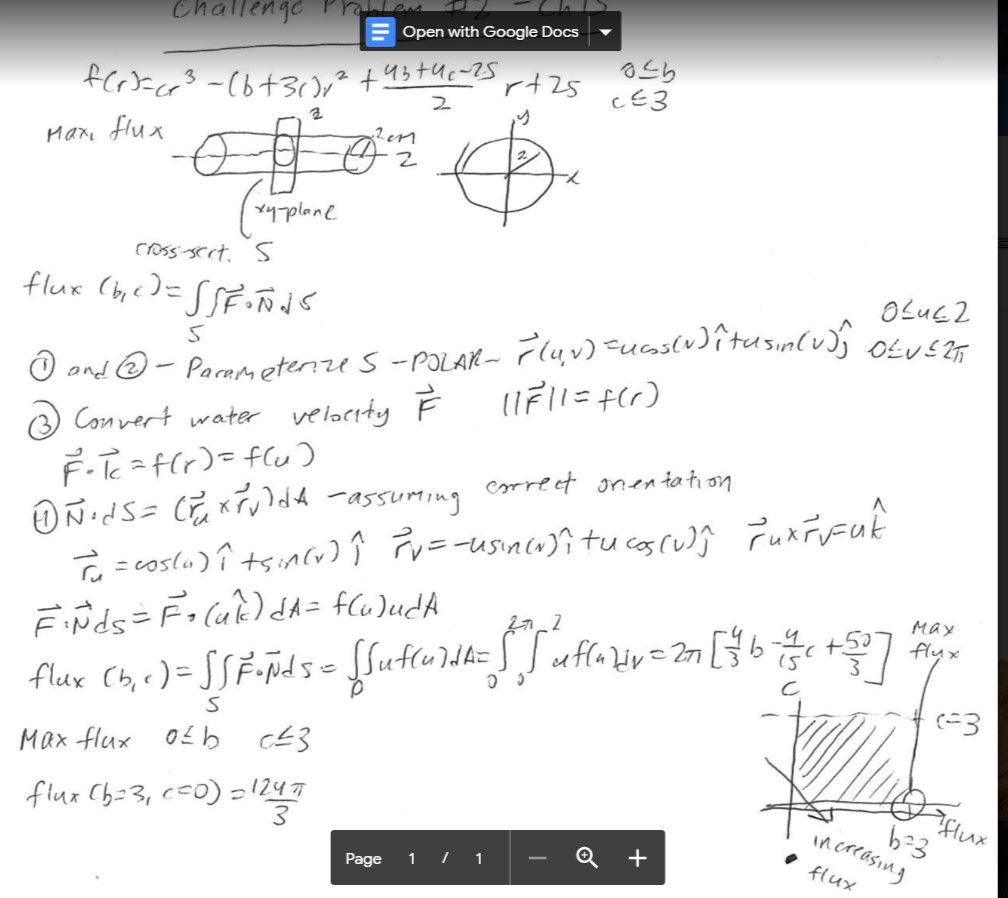
\includegraphics[]{Cp2diagram.jpg}

\end{document}
